\documentclass[11pt,letterpaper]{article}
\usepackage[utf8]{inputenc}
\usepackage[top=1in,bottom=1in,left=1in,right=1in]{geometry}
\usepackage{amsmath}
\usepackage{amsfonts}
\usepackage{amssymb}
\usepackage{amsthm}
\usepackage{bm}
\usepackage{braket}
\usepackage{cancel}
\usepackage{enumitem}
\usepackage{float}
\usepackage{forloop}
\usepackage{graphicx}
\usepackage{hyperref}
\usepackage{mathabx}
\usepackage{parskip}
\usepackage{subcaption}
\usepackage{tensor}
\usepackage{titlesec}
\usepackage{titling}


\setenumerate{leftmargin=*}


% \titlelabel{(\thetitle)\quad}
\titleformat*{\section}{\large\bfseries}
\titleformat*{\subsection}{\normalsize\bfseries}
\setlength{\droptitle}{-5em}


\DeclareMathOperator*{\argmin}{arg\,min}
\DeclareMathOperator*{\argmax}{arg\,max}

\DeclareMathOperator{\tr}{tr}

\let\Re\relax
\DeclareMathOperator{\Re}{Re}
\let\Im\relax
\DeclareMathOperator{\Im}{Im}

\DeclareMathOperator{\sgn}{sgn}

\newcommand{\R}{\mathbb{R}}


\theoremstyle{definition}
\newtheorem{defn}{Definition}[section]

\theoremstyle{plain}
\newtheorem{thm}{Theorem}[section]



\newcommand{\bhat}[1]{\hat{\bm{#1}}}


\renewcommand{\thesubsection}{\normalsize \alph{subsection}}
\renewcommand{\d}{\mathrm{d}}
\renewcommand{\vec}[1]{\bm{#1}}
\newcommand{\del}{\vec{\nabla}}
\newcommand{\e}{\epsilon}
\newcommand{\tpd}[3]{\left( \frac{\partial #1}{\partial #2} \right)_{#3}}
\newcommand{\pd}[2]{\frac{\partial #1}{\partial #2}}
\newcommand{\spd}[2]{\frac{\partial^2 #1}{\partial {#2}^2}}
\def\dbar{{\mathchar'26\mkern-12mu d}}

\allowdisplaybreaks


\author{Sam Kowash}
\numberwithin{equation}{section}
\numberwithin{figure}{section}
\title{CSE 546 HW \#3}

\begin{document}
\maketitle

\section{Bayesian Inference}
\begin{enumerate}
	\item \begin{enumerate}
		\item
		\item 
		\item 
		\item 
		\item 
	\end{enumerate}






	\item \begin{enumerate}
		\item
		\item 
	\end{enumerate}
\end{enumerate}
































\section{Kernel Regression}
\begin{enumerate}
\setcounter{enumi}{2}
	\item \begin{enumerate}
		\item
		\item 
		\item 
		\item 
		\item 
	\end{enumerate}
\end{enumerate}




















\section{\texorpdfstring{$k$-means clustering}{k-means clustering}}
\begin{enumerate}
\setcounter{enumi}{3}
	\item \begin{enumerate}
		\item Figures below show cluster centers in the full MNIST set (train joined with test) from $k$-means for a variety of different cluster counts. In general, they all resemble identifiable numerals, but more clusters tends to lead to more distinct features. At $k=5$ we see centers somewhere in between similar numerals like 3 and 8 or 9 and 4, but at $k=20$ the algorithm has the freedom to center clusters around more specific forms like taller or rounder or more slanted 9s.


		\begin{figure}[H]
			\centering
			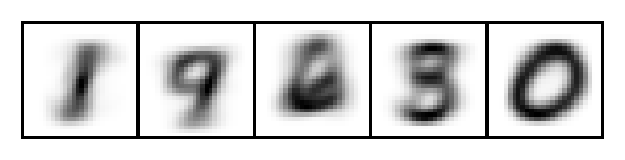
\includegraphics[width=.5\textwidth]{figures/5-centers.pdf}
			\caption{Final centers for $k=5$ with uniform initialization}
		\end{figure}

		\begin{figure}[H]
			\centering
			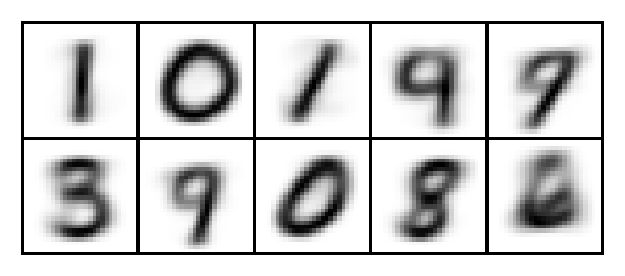
\includegraphics[width=.5\textwidth]{figures/10-centers.pdf}
			\caption{Final centers for $k=10$ with uniform initialization}
		\end{figure}

		\begin{figure}[H]
			\centering
			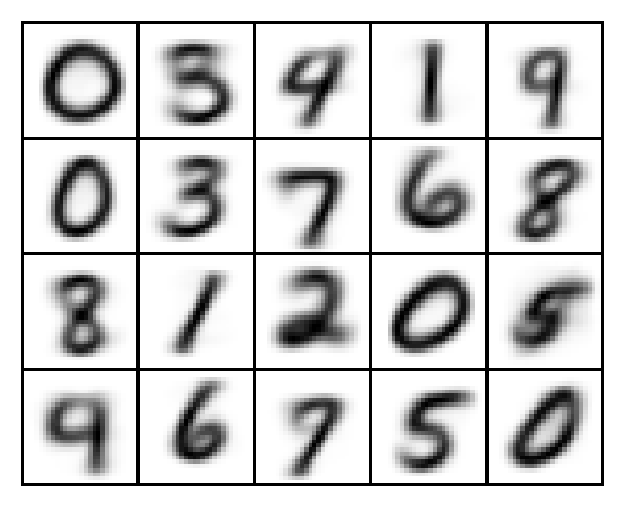
\includegraphics[width=.5\textwidth]{figures/20-centers.pdf}
			\caption{Final centers for $k=20$ with uniform initialization}
		\end{figure}




		\item Figures below show centers obtained with the $\texttt{k-means++}$ intialization scheme. They look broadly similar to the uniform case, although perhaps modestly crisper. 

		Fig.~\ref{fig:km_objs} compare the convergence rate to uniform initialization through the mean squared distance from a point to its cluster center. We see that other than for $k=5$, the new initialization converges faster and to smaller mean distances.

		\begin{figure}[H]
			\centering
			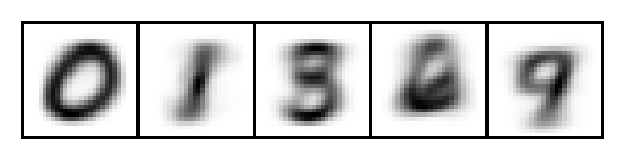
\includegraphics[width=.5\textwidth]{figures/5pp-centers.pdf}
			\caption{Final centers for $k=5$ with \texttt{k-means++} initialization}
		\end{figure}

		\begin{figure}[H]
			\centering
			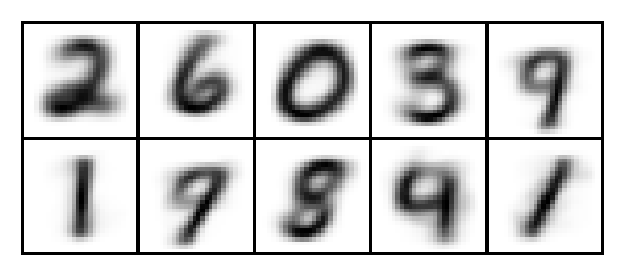
\includegraphics[width=.5\textwidth]{figures/10pp-centers.pdf}
			\caption{Final centers for $k=10$ with \texttt{k-means++} initialization}
		\end{figure}

		\begin{figure}[H]
			\centering
			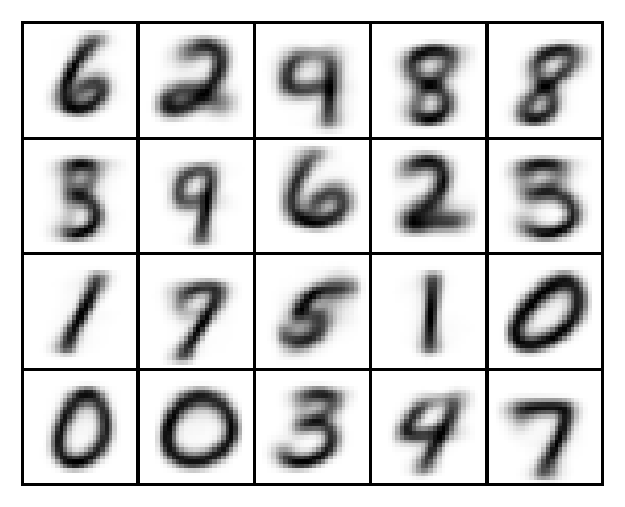
\includegraphics[width=.5\textwidth]{figures/20pp-centers.pdf}
			\caption{Final centers for $k=20$ with \texttt{k-means++} initialization}
		\end{figure}


		\begin{figure}[H]
		\centering
			\begin{subfigure}[t]{.32\textwidth}
				\centering
				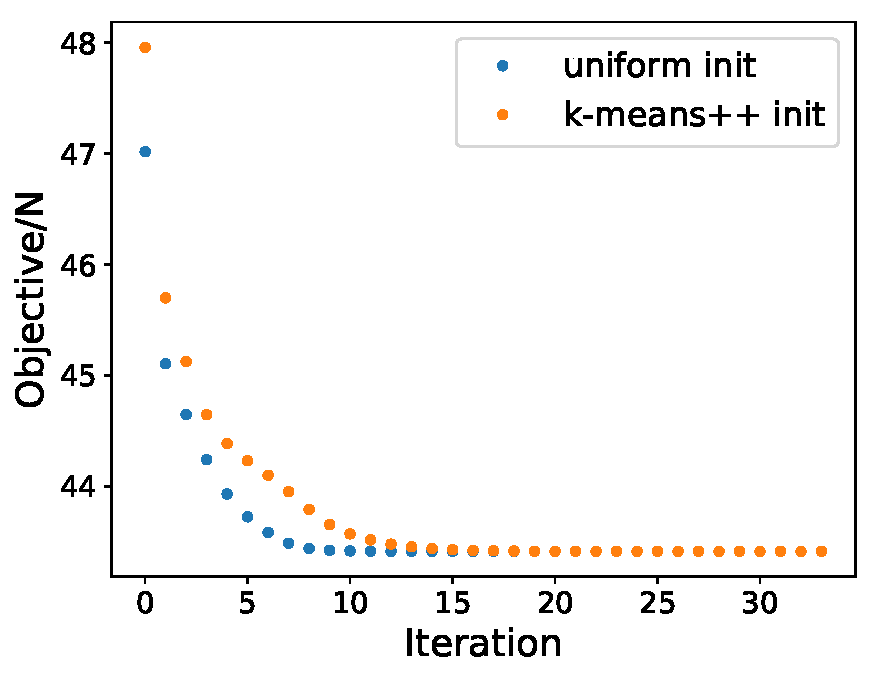
\includegraphics[width=\textwidth]{figures/5-objective.pdf}
			\end{subfigure}
			%
			\begin{subfigure}[t]{.32\textwidth}
				\centering
				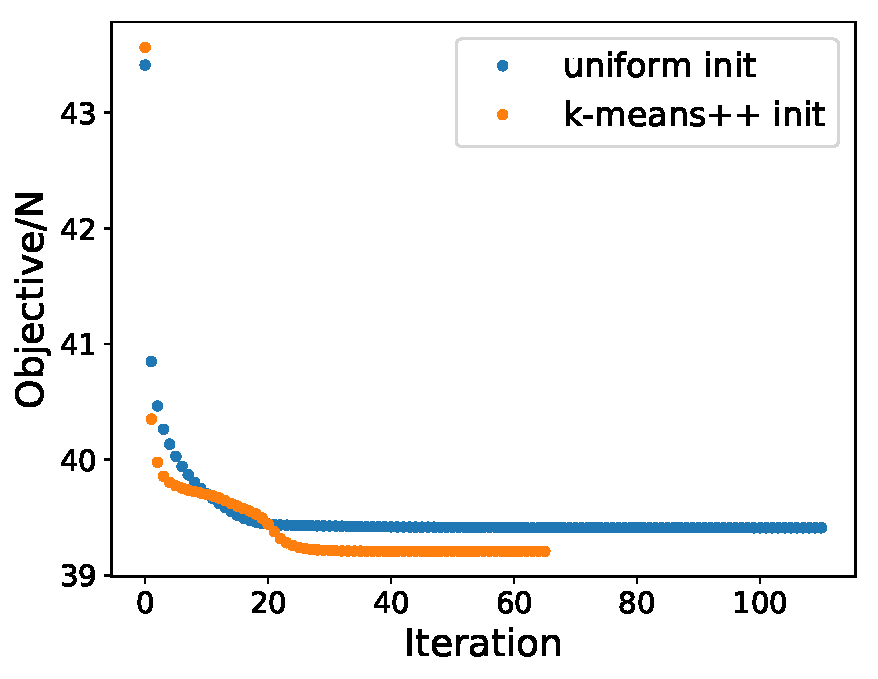
\includegraphics[width=\textwidth]{figures/10-objective.pdf}
			\end{subfigure}
			%
			\begin{subfigure}[t]{.32\textwidth}
				\centering
				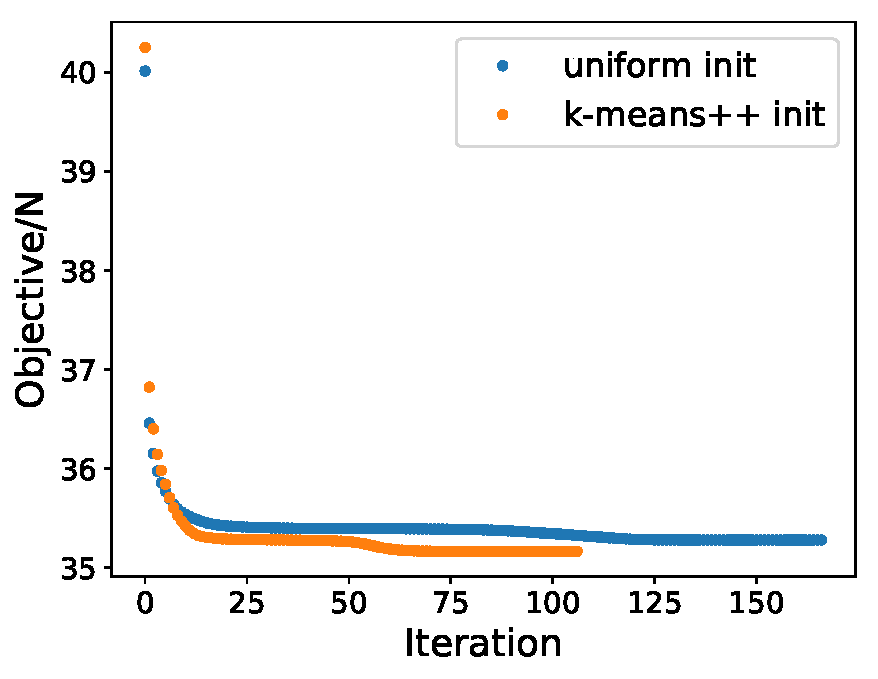
\includegraphics[width=\textwidth]{figures/20-objective.pdf}
			\end{subfigure}

			\caption{Objective function vs. iteration number for $k = 5,10,20$ from left to right}
		\end{figure}
		\label{fig:km_objs}
	\end{enumerate}
\end{enumerate}
















\section{Joke Recommender System}
\begin{enumerate}
\setcounter{enumi}{4}
	\item \begin{enumerate}
		\item
		\item 
		\item 
	\end{enumerate}
\end{enumerate}

\end{document}